%!TEX root = draft.tex
\section{Scaling results} \label{sec:scaling}
In this section we present some results that demonstrate the scalability of our algorithms. All of our tests were ran on the Stampede cluster at the Texas Advanced Computing Center (TACC) where we are limited to $4096$ cores at most. Each node of Stampede has 2 eight-core Xenon E5-2680 processes clocked at 2.7 GHz with 32 GB of DDR3-1600 MHz memory and interconnected using an InfiniBand network card. Unless mentioned otherwise, in all the tests we have used all 16 cores of every node. Finally, in all cases we report the maximum wall time recorded using PETSc's logging interface which has a temporal resolution of roughly $0.1 \: \mu s$.

We define parallel efficiency as $e=s\cdot P_1 / P$ where $s=t_1/t_P$ is the speed-up, $P_1$ is the smallest number of processes for which the test was run, $t_1$ is the time to run the problem on $P_1$ processes, $P$ is the number of processes and $t_P$ is the time to run the problem on $P$ processes. We note that efficiencies larger than $100\%$ are reported for some cases. This is common and can be hardware related, for instance linked to the problem being locally smaller for larger number of processes and thus exploiting the cache better.

\subsection{Interpolation}
In this section we show the results for a simple test to measure the scalability of the interpolation Algorithm \ref{alg:interpolation}. The test consists of interpolating a function at a number of random points on a randomly refined Octree in three spatial dimensions. We consider two cases, a small test on a level\footnote{The level is the number of recursive splits allowed for each tree.} 9 tree with roughly 33M nodes and a larger test on a level 13 tree with roughly 280M nodes. In both cases the number of randomly generated points is chosen to be equal to the number of nodes and the stabilized second-order interpolation of \cite{Min;Gibou:07:A-second-order-accur} is performed 10 times to smooth out possible timing fluctuations.

To simulate the effect of different CFL numbers, we generate the random points such that on each process $\alpha$ percentage of them are located outside the process boundary and thus will initiate communication. Scaling results are presented for $\alpha = 5 \%$ and $\alpha = 95\%$ for both the small and large problems in Figure \ref{fig:interpolation}. We also present a third row of results for a much larger problem with roughly 1.66B nodes on a level 14 tree. Excellent scaling is obtained for the small problem for $P = 16-512$ even when $95\%$ of the interpolation points belong to a remote process. For the larger problem, however, the communication overhead prevents the algorithm from scaling beyond $2048$ processes when $\alpha = 95\%$ (cf.\ Table \ref{tab:scaling_interpolation}). Note, however, that this is expected since the total time is dominated by communication for $\alpha = 95\%$ and there is very little local work in this case. Indeed, the last row of Figure \ref{fig:interpolation} show much better scaling behavior on a larger problem size, e.g. efficiencies are increased from $e=34\%$ to $e=68\%$ for $\alpha = 95\%$ on 4096 processes. This is a typical result with strong scaling and simply implies that our algorithms are scalable for sufficiently large problems.
\begin{figure}[htbp]
	\begin{center}
		\subfigure[$N_G = 33$M, $\alpha = 5\%$]{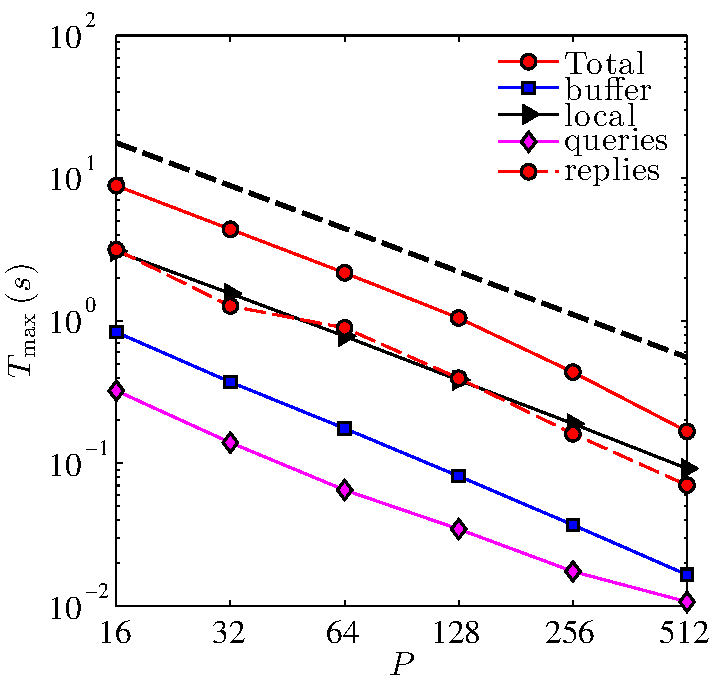
\includegraphics[width = 0.38 \textwidth] {figures/host_Interpolation_small_alpha_5.pdf}} \hspace{0.5 in}
		\subfigure[$N_G = 33$M, $\alpha = 95\%$]{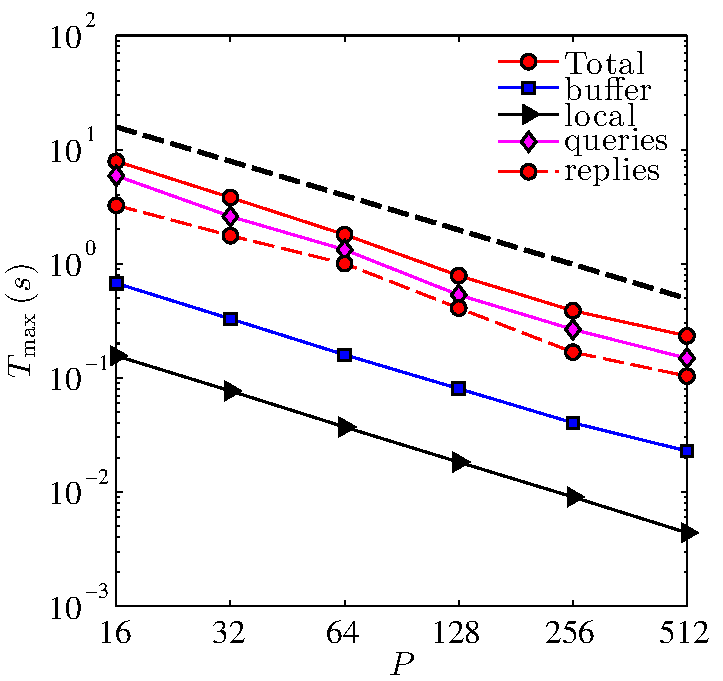
\includegraphics[width = 0.38 \textwidth] {figures/host_Interpolation_small_alpha_95.pdf}}
		\\
		\subfigure[$N_G = 280$M, $\alpha = 5\%$]{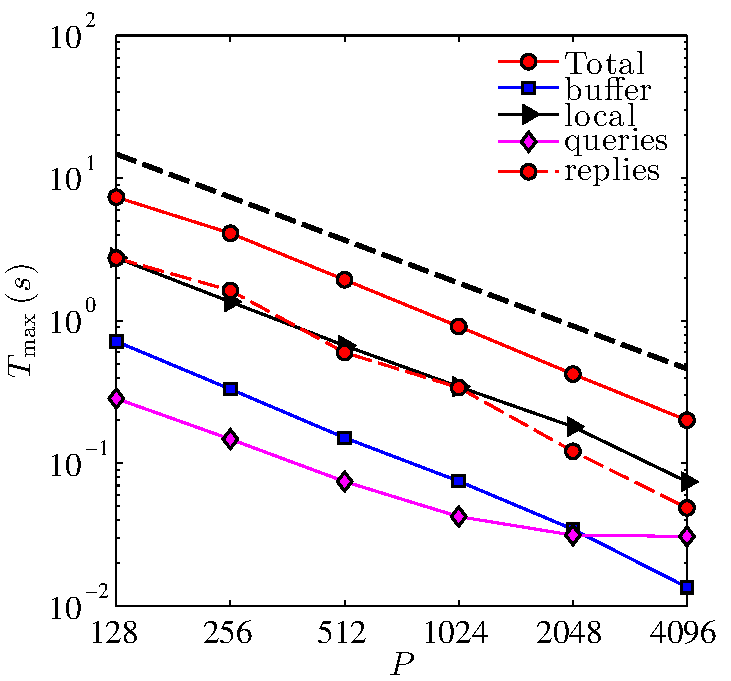
\includegraphics[width = 0.38 \textwidth] {figures/host_Interpolation_large_alpha_5.pdf}} \hspace{0.5 in}
		\subfigure[$N_G = 280$M, $\alpha = 95\%$]{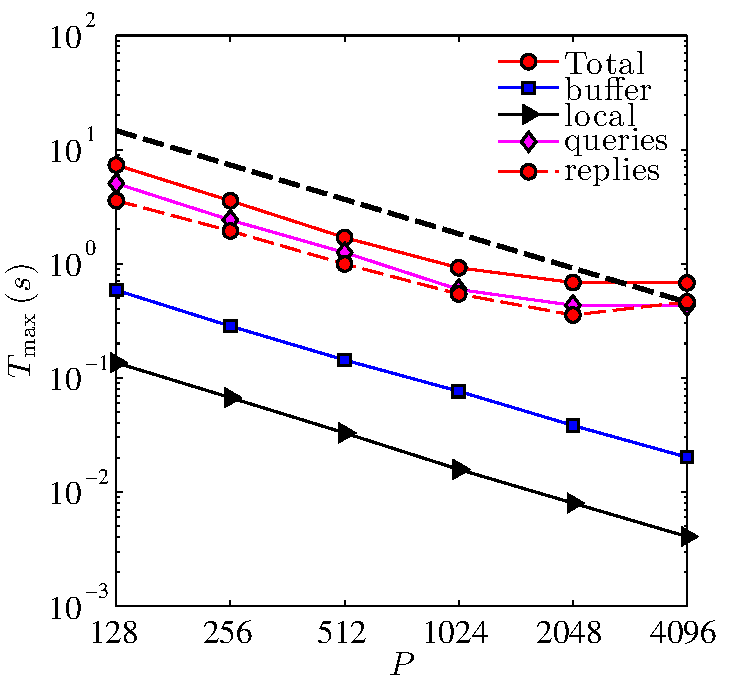
\includegraphics[width = 0.38 \textwidth] {figures/host_Interpolation_large_alpha_95.pdf}}
		\\
		\subfigure[$N_G = 1.66$B, $\alpha = 50\%$]{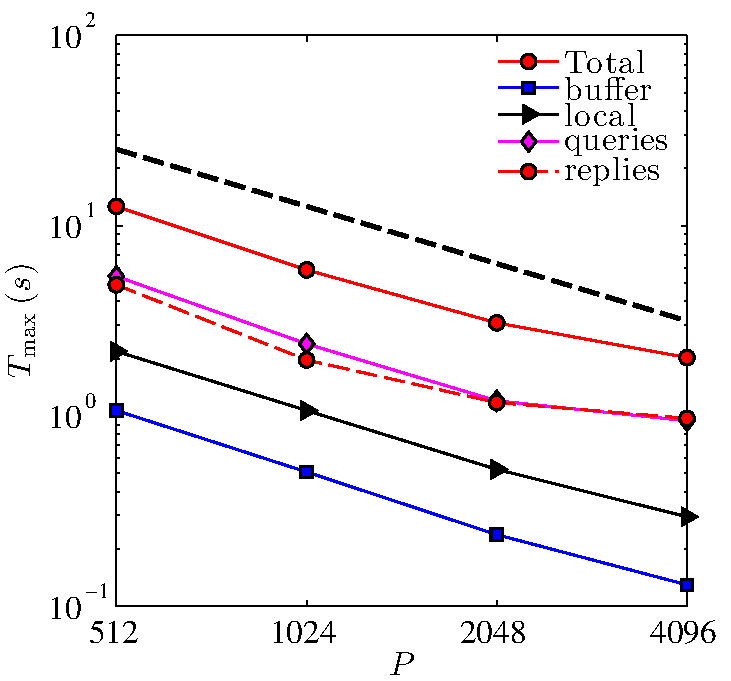
\includegraphics[width = 0.38 \textwidth] {figures/host_Interpolation_super_large_alpha_50.pdf}} \hspace{0.5 in}
		\subfigure[$N_G = 1.66$B, $\alpha = 95\%$]{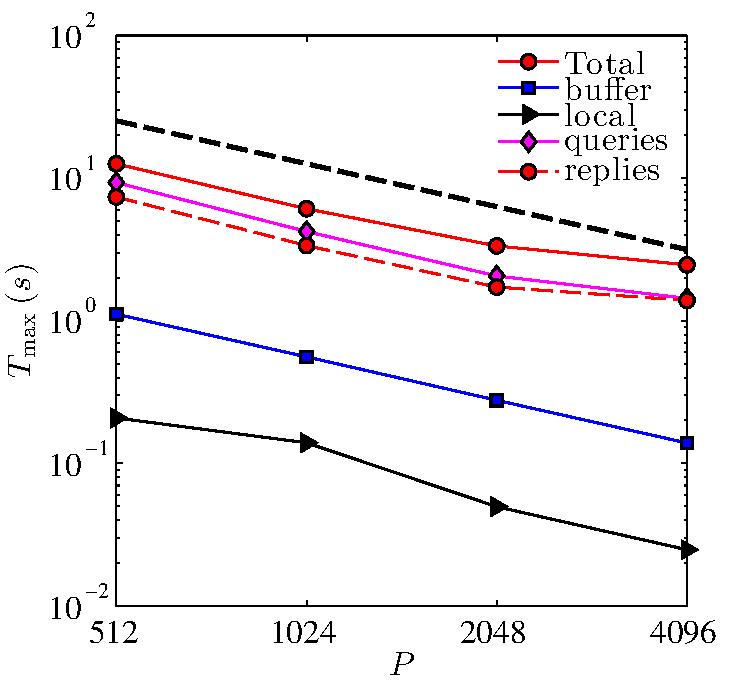
\includegraphics[width = 0.38 \textwidth] {figures/host_Interpolation_super_large_alpha_95.pdf}}
	\end{center}
	\caption{Strong scaling of Algorithm \ref{alg:interpolation} for several tests where $N_G$ denotes the number of random interpolation points (which is the same as the number of nodes in the Octree) and $\alpha$ denotes the percentage of these points that are remote for each process. Here ``Total'' represents the total time spent in the interpolation while ``buffer'', ``local'', ``queries'', and ``replies'' represent the the timing for different sections (cf.\ Algorithm \ref{alg:interpolation}). The black dashed line represents the ideal scaling. The results indicate excellent scaling for the small test (a-b) and for the large test when $\alpha = 5\%$ (c). For the extreme case (d) the algorithm stops scaling at $2048$ processes due to communication overhead. Note, however, that this merely indicates that the problem size is not large enough for this test case. Indeed much better scaling is obtained when the problem size is increased to $N_G = 1.66$B points (e-f).}
	\label{fig:interpolation}
\end{figure}

\begin{table}[ht!]
\centering
	\begin{tabular}{|l|l|cccccc|}
	\hline
	\multirow{3}{*}{Small Test} & \multicolumn{1}{|c|}{$P$} & 16      & 32      & 64      & 128     & 256    & 512 \\
	\cline{2-8} 	                            
	                            & $\alpha = 5\%$   & $100\%$ & $101\%$ & $102\%$ & $106\%$ & $127\%$& $165\%$ \\
	                            & $\alpha = 95\%$  & $100\%$ & $104\%$ & $110\%$ & $125\%$ & $127\%$& $106\%$ \\ 	                            
	\hline
	\multirow{3}{*}{Large Test} & \multicolumn{1}{|c|}{$P$} & 128     & 256     & 512     & 1024    & 2048   & 4096 \\
	\cline{2-8} 	                            
	                            & $\alpha = 5\%$   & $100\%$ & $89\%$  & $95\%$  & $101\%$ & $109\%$& $114\%$ \\
	                            & $\alpha = 95\%$  & $100\%$ & $103\%$ & $108\%$ & $99\%$  & $67\%$ & $34\%$ \\
	\hline
	\multirow{3}{*}{Very Large Test} & \multicolumn{1}{|c|}{$P$} & 128     & 256     & 512     & 1024    & 2048   & 4096 \\
	\cline{2-8} 	                            
	                            & $\alpha = 50\%$  & -- & -- & $100\%$ & $108\%$ & $102\%$& $78\%$ \\
	                            & $\alpha = 95\%$  & -- & -- & $100\%$ & $103\%$ & $94\%$ & $64\%$ \\
	\hline
	\end{tabular}
	\caption{Parallel efficiency of the total runtime of the interpolation algorithm for the small (33M nodes), large (280M nodes), and very large (1.66B nodes) tests. Reported efficiencies are based on the lowest number of processes for each test.}
	\label{tab:scaling_interpolation}
\end{table}

\subsection{Semi-Lagrangian}
To test the scalability of the semi-Lagrangian scheme of Algorithm \ref{alg:semi-lagrangian}, we consider a slightly modified version of the Enright's rotation test \cite{Enright;Fedkiw;Ferziger;etal:02:A-Hybrid-Particle-Le}, i.e. we advect a sphere of radius 0.35 located at $(0.4, 0.4, 0.4)$ with a divergence free velocity field given by:
\bean
u(x,y,z) &=& 2\sin(\pi x)^2 \sin(2\pi y) \sin(2 \pi z), \\
v(x,y,z) &=& -\sin(\pi y)^2 \sin(2\pi x) \sin(2 \pi z),\\
w(x,y,z) &=& -\sin(\pi z)^2 \sin(2\pi x) \sin(2 \pi y). 
\eean
To understand the effect of the CFL number on the scalability of the algorithm we perform one step of the semi-Lagrangian algorithm for $\text{CFL} = 1$, $\text{CFL} = 10$, and $\text{CFL} = 100$. We also perform the test for two different initial girds, a small grid with maximum level $l_\text{max} = 10$ and a large grid with maximum level $l_\text{max} = 12$. In both cases, the minimum level is $l_\text{min}=0$. After one advection step, these grids have approximately 15M and 255M nodes, respectively. 
\begin{table}[htbp]
	\begin{minipage}{.48\linewidth}
		\begin{center}
		\begin{tabular}{|c|cccccc|}
			\hline
				\diagbox{CFL}{\#p} & 16 & 32 & 64 & 128 & 256 & 512 \\
				\hline
				1   & 2 & 2 & 3 & 3 & 3 & 3 \\
				10  & 3 & 3 & 3 & 3 & 3 & 3 \\
				100 & 6 & 6 & 6 & 6 & 6 & 6 \\
			\hline
		\end{tabular}
		\caption*{(a) $l_\text{max} = 10$}
		\end{center}
	\end{minipage}%
	\begin{minipage}{.48\linewidth}
		\begin{center}
		\begin{tabular}{|c|cccccc|}
			\hline
				\diagbox{CFL}{\#p} & 128 & 256 & 512 & 1024 & 2048 & 4096 \\
			\hline
				1   & 3 & 3 & 3 & 3 & 3 & 3 \\
				10  & 3 & 3 & 4 & 4 & 4 & 4 \\
				100 & 6 & 6 & 6 & 6 & 6 & 7 \\
			\hline
		\end{tabular}
		\caption*{(b) $l_\text{max} = 12$}
		\end{center}
	\end{minipage}	
	\caption{Number of sub-iterations required for the grid construction in Algorithm \ref{alg:semi-lagrangian} for the rotation test on a (a) level-10 and (b) level-12 Octree with approximately 15M and 255M nodes, respectively. Note how the sub-iteration count increases with the CFL number but is almost independent of the number of processes. The slight dependence between the number of sub-iterations and the number of processes is most likely due to the dependence of round-off errors on the number of processes. Nonetheless, close examination of the Octrees generated (data not shown) reveals that they are identical and independent of the number of processes used to perform the test.}
	\label{tab:semilagrangian}
\end{table}

Unlike many existing applications where the mesh is changed infrequently, our semi-Lagrangian algorithm requires several sub-iterations of the refinement and coarsening operations. As a result, it is expected that refinement and coarsening steps constitute a significant portion of the total runtime which puts stringent scalability requirements on these algorithms. We refer the interested reader to section 3.2 of \cite{Burstedde;Wilcox;Ghattas:11:p4est:-Scalable-Algo} for detailed description of scalable refinement and coarsening algorithms in \texttt{p4est}. 

Table \ref{tab:semilagrangian} illustrates the dependence of the number of sub-iterations required to build the grid on the CFL number; as the CFL is increased, the interface travels a farther distance, which necessitates more sub-iterations to generate the grid. Figures \ref{fig:semilagrangian_small} and \ref{fig:semilagrangian_large} illustrate the scalability of the algorithm for the small and large problems, respectively. To enable meaningful comparisons between different CFL numbers and number of processes, the maximum time has been scaled by the number of sub-iterations required for the grid construction as reported in Table \ref{tab:semilagrangian}. For both problems, excellent scalability is observed for $\text{CFL} = 1$ and $\text{CFL} = 10$. The algorithm even shows good scalability when taken to the extreme, i.e. for $\text{CFL} = 100$.

An increase in the CFL number has two effects on the algorithm. First, a larger fraction of the departure points lands in the domains of remote processes. Moreover, these points are potentially dispersed across a larger number of processes. This means that the communication volume should increase with the CFL number. Second, as more points are shipped to remote processes for interpolation, there is a greater chance that the interpolation load is imbalanced across processes. This is especially true for regions of space in which the streamlines cluster. Both factors can contribute to reducing the scalability of the algorithm at large CFL numbers. 
\begin{figure}[htbp]
	\begin{center}
		\subfigure[semi-Lagrangian, $\text{CFL} = 1$]{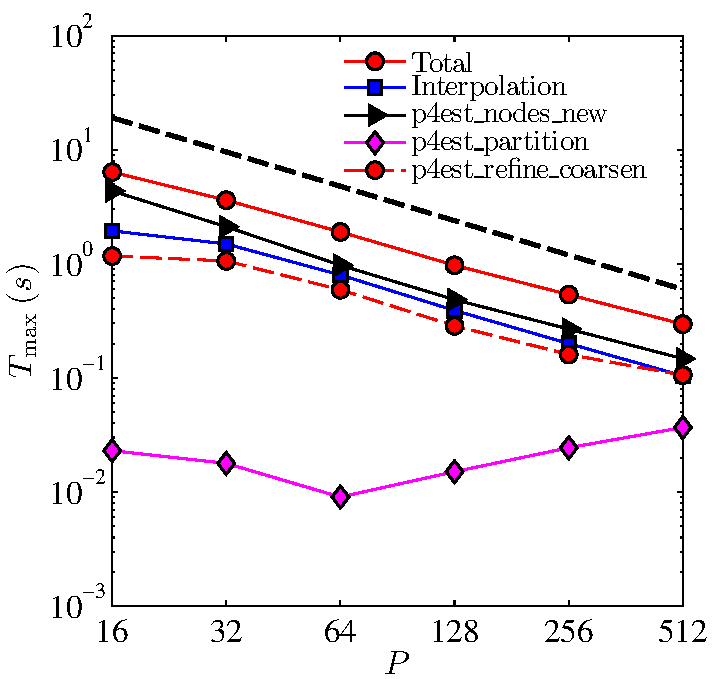
\includegraphics[width = 0.32 \textwidth] {figures/host_SemiLagrangian_small_CFL_1.pdf}}
		\subfigure[semi-Lagrangian, $\text{CFL} = 10$]{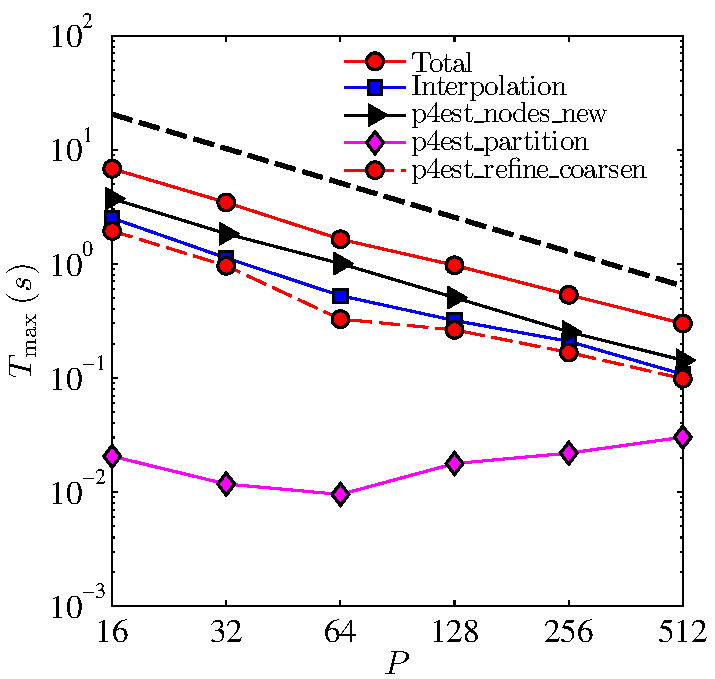
\includegraphics[width = 0.32 \textwidth] {figures/host_SemiLagrangian_small_CFL_10.pdf}}
		\subfigure[semi-Lagrangian, $\text{CFL} = 100$]{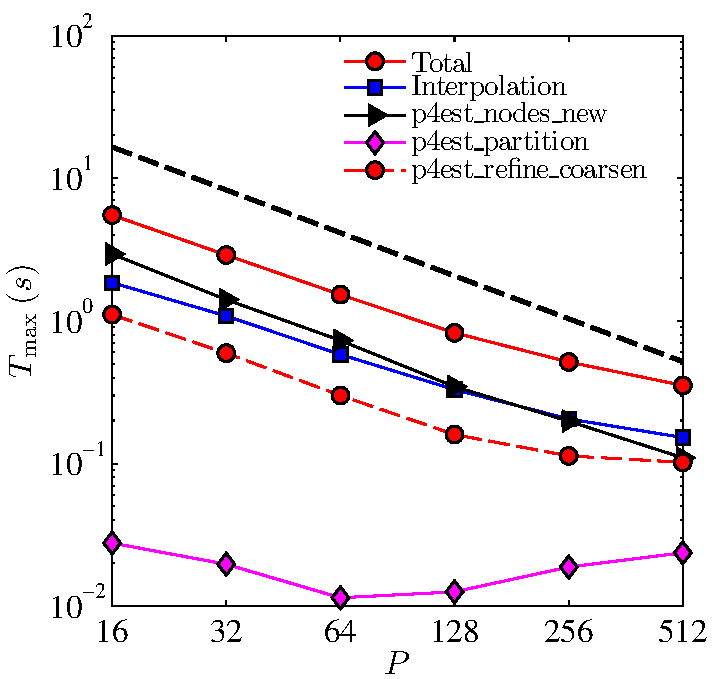
\includegraphics[width = 0.32 \textwidth] {figures/host_SemiLagrangian_small_CFL_100.pdf}}
		\\
		\subfigure[Interpolation, $\text{CFL} = 1$]{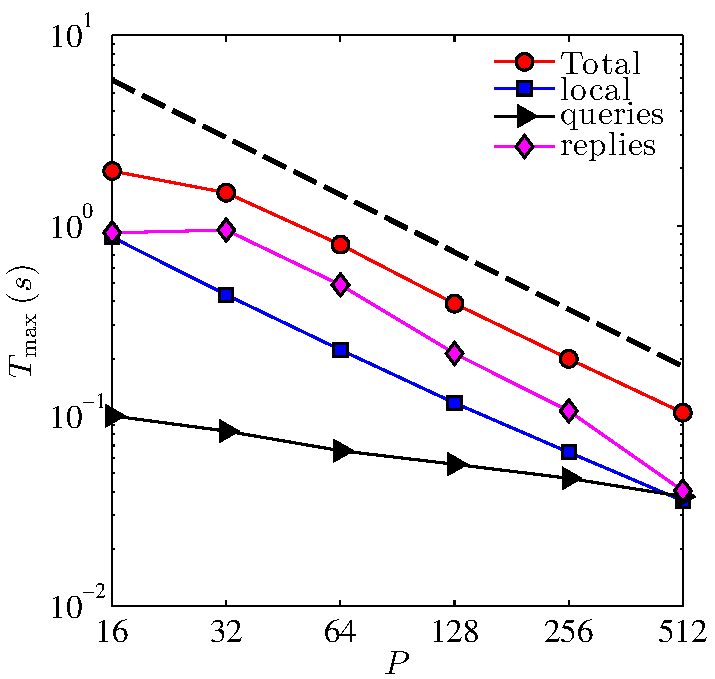
\includegraphics[width = 0.32 \textwidth] {figures/host_SemiLagrangian_Interpolation_small_CFL_1.pdf}}
		\subfigure[Interpolation, $\text{CFL} = 10$]{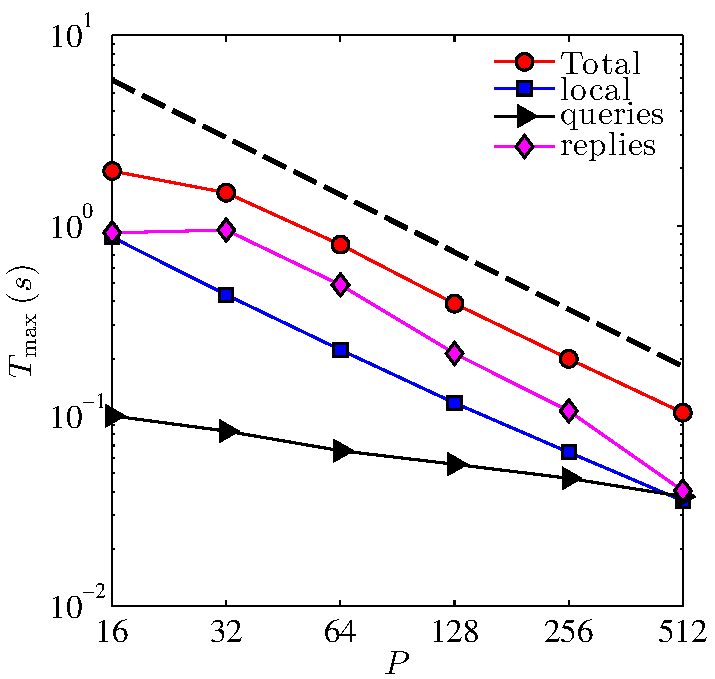
\includegraphics[width = 0.32 \textwidth] {figures/host_SemiLagrangian_Interpolation_small_CFL_1.pdf}}
		\subfigure[Interpolation, $\text{CFL} = 100$]{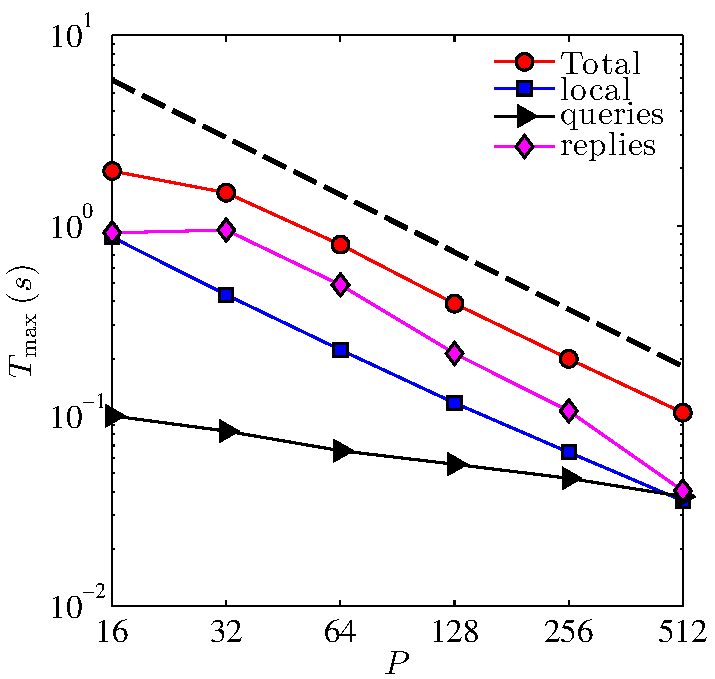
\includegraphics[width = 0.32 \textwidth] {figures/host_SemiLagrangian_Interpolation_small_CFL_1.pdf}}
	\end{center}
	\caption{Strong scaling of a single time step of Algorithm \ref{alg:semi-lagrangian} for the rotation test on a level-10 Octree with approximately 15M nodes. Top row: scaling of the various components of the algorithm for (a) $\text{CFL} = 1$, (b) $\text{CFL} = 10$, and (c) $\text{CFL} = 100$. Bottom row: breakdown of the various components of the interpolation phase for the same CFL numbers. The solid dashed line represents the ideal scaling. Note that the maximum time has been scaled by the number of sub-iterations required to build the tree (cf.\ Table \ref{tab:semilagrangian}). Here \texttt{p4est\_nodes\_new}, \texttt{p4est\_partition} and \texttt{p4est\_refine\_coarsen} refer to constructing the global indexing for nodes, partitioning the forest, and the refining/coarsening operation, respectively \cite{Burstedde;Wilcox;Ghattas:11:p4est:-Scalable-Algo}.}
	\label{fig:semilagrangian_small}
\end{figure}

\begin{figure}[htbp]
	\begin{center}
		\subfigure[semi-Lagrangian, $\text{CFL} = 1$]{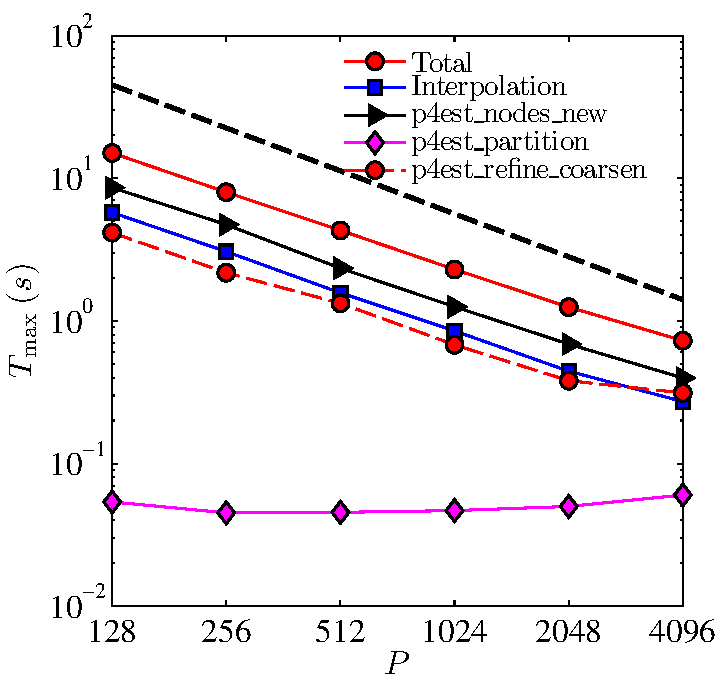
\includegraphics[width = 0.32 \textwidth] {figures/host_SemiLagrangian_large_CFL_1.pdf}}
		\subfigure[semi-Lagrangian, $\text{CFL} = 10$]{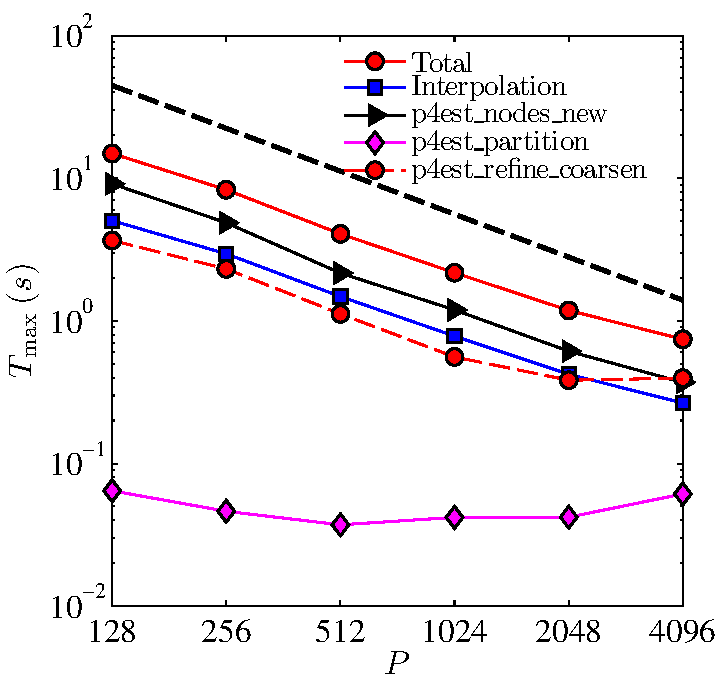
\includegraphics[width = 0.32 \textwidth] {figures/host_SemiLagrangian_large_CFL_10.pdf}}
		\subfigure[semi-Lagrangian, $\text{CFL} = 100$]{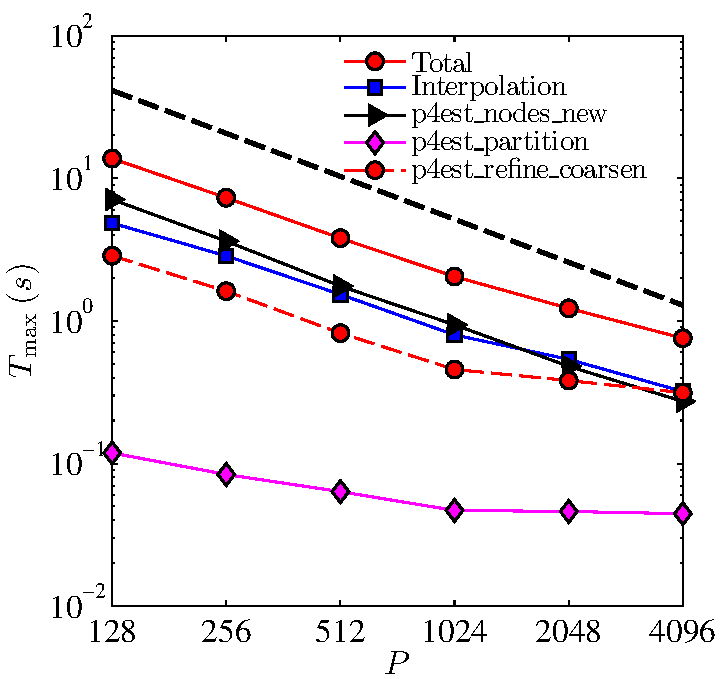
\includegraphics[width = 0.32 \textwidth] {figures/host_SemiLagrangian_large_CFL_100.pdf}}
		\\
		\subfigure[Interpolation, $\text{CFL} = 1$]{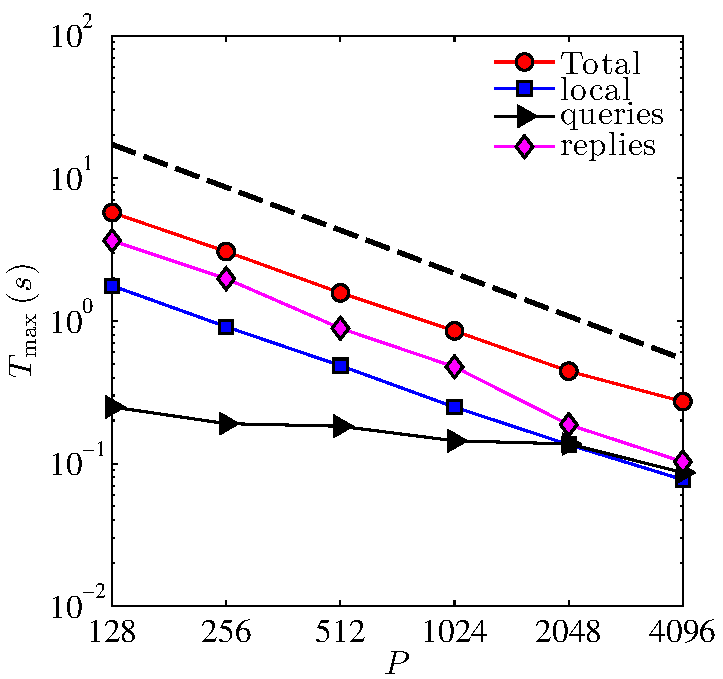
\includegraphics[width = 0.32 \textwidth] {figures/host_SemiLagrangian_Interpolation_large_CFL_1.pdf}}
		\subfigure[Interpolation, $\text{CFL} = 10$]{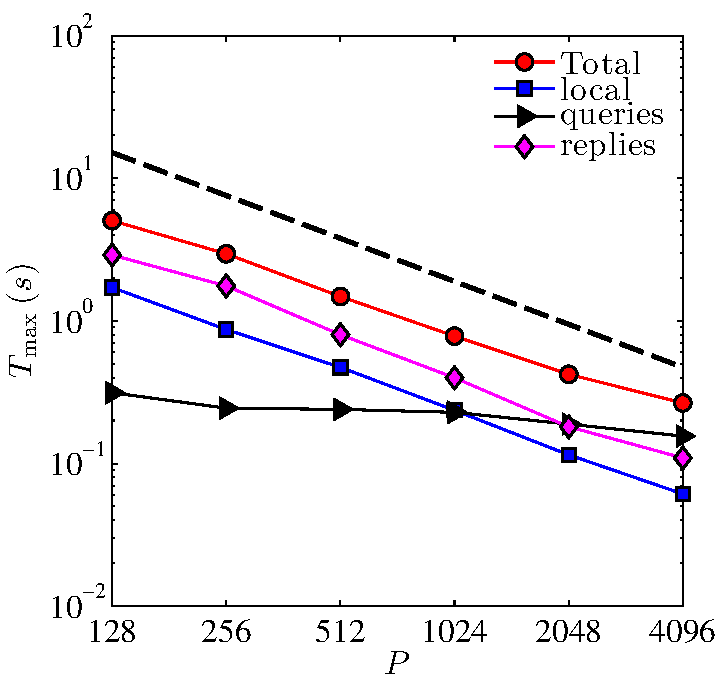
\includegraphics[width = 0.32 \textwidth] {figures/host_SemiLagrangian_Interpolation_large_CFL_10.pdf}}
		\subfigure[Interpolation, $\text{CFL} = 100$]{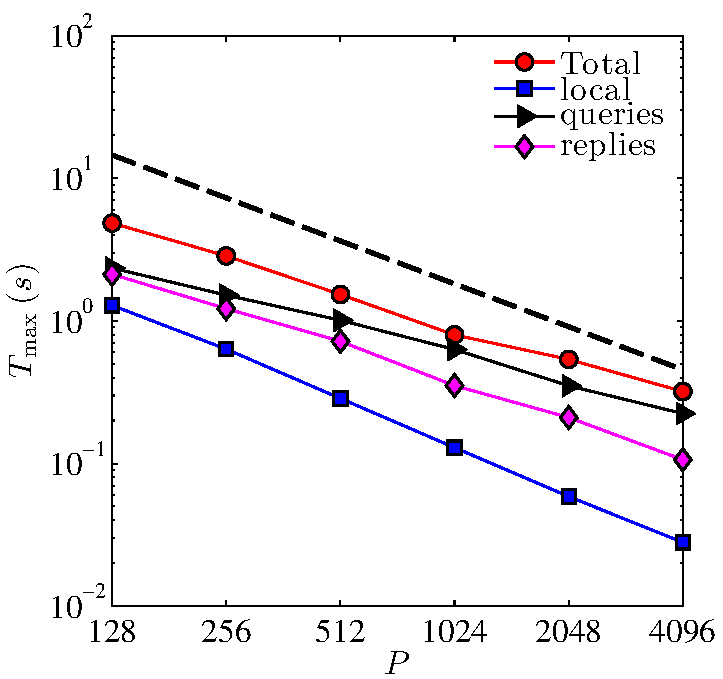
\includegraphics[width = 0.32 \textwidth] {figures/host_SemiLagrangian_Interpolation_large_CFL_100.pdf}}
	\end{center}
	\caption{Strong scaling of a single time step of Algorithm \ref{alg:semi-lagrangian} for the rotation test on a level-12 Octree with approximately 255M nodes. Top row: scaling of the various components of the algorithm for (a) $\text{CFL} = 1$, (b) $\text{CFL} = 10$, and (c) $\text{CFL} = 100$. Bottom row: breakdown of the various components of the interpolation phase for the same CFL numbers. The solid dashed line represents the ideal scaling. Note that the maximum time has been scaled by the number of sub-iterations required to build the tree (cf.\ Table \ref{tab:semilagrangian}).}
	\label{fig:semilagrangian_large}
\end{figure}

\begin{table}
\centering
	\begin{tabular}{|l|l|cccccc|}
	\hline
	\multirow{4}{*}{Small Test} & \multicolumn{1}{|c|}{$P$} & 16      & 32      & 64      & 128     & 256    & 512 \\
	\cline{2-8} 	                            
	                            & $\text{CFL} = 1$   & $100\%$ & $88\%$  & $84\%$  & $82\%$  & $74\%$ & $67\%$ \\
	                            & $\text{CFL} = 10$  & $100\%$ & $99\%$  & $104\%$ & $88\%$  & $80\%$ & $71\%$ \\ 	                            
	                            & $\text{CFL} = 100$ & $100\%$ & $95\%$  & $90\%$  & $84\%$  & $67\%$ & $49\%$ \\
	\hline
	\multirow{4}{*}{Large Test} & \multicolumn{1}{|c|}{$P$} & 128     & 256     & 512     & 1024    & 2048   & 4096 \\
	\cline{2-8} 	                            
	                            & $\text{CFL} = 1$   & $100\%$ & $94\%$  & $87\%$  & $82\%$  & $75\%$ & $65\%$ \\
	                            & $\text{CFL} = 10$  & $100\%$ & $90\%$  & $92\%$  & $86\%$  & $79\%$ & $63\%$ \\
	                            & $\text{CFL} = 100$ & $100\%$ & $94\%$  & $90\%$  & $84\%$  & $70\%$ & $57\%$ \\
	\hline
	\end{tabular}
	\caption{Parallel efficiency of the runtime of a single semi-Lagrangian step. Reported efficiencies are based on the lowest number of processes for each test.}
	\label{tab:scaling_semilagrangian}
\end{table}

To better understand the importance of the CFL number on the scalability, we have recorded a complete history of the communication pattern in the interpolation step. Figure \ref{fig:communication_4096} illustrates the effects of the CFL number on different metrics, namely the number of interpolation points\footnote{Note that this includes both the local points and the points queried by other processes.}, $N_p$, the number of sent and received messages, $N_m = S + R$, and the total communication volume, $V_m$ in megabytes (MB), for $p=4096$ processes. Furthermore, these values are reported for the first (top row) and last (bottom row) sub-iterations of the semi-Lagrangian algorithm. There are several points to make. First, increasing the CFL number greatly increases the load imbalance, as shown by the spread of the data in Figure \ref{fig:communication_4096_pf}. This is because at higher CFL numbers, it is more likely that some processes will receive a larger portion of the backtracked points. Second, increasing the CFL number increases both the communication volume and its spread across processes (cf.\ Figure \ref{fig:communication_4096_vf}). Interestingly, however, the number of sent and received messages do not seem to be affected by the CFL number. The bottom row of Figure \ref{fig:communication_4096} exhibits a better balance both in the computation and communication volume in the last sub-iteration of the semi-Lagrangian algorithm. This can be justified by noting that for the final sub-iteration, the partitioning of $G^{n+1}$ is more consistent with the partitioning of the departure points on $G^n$. Detailed information about the load balancing and the communication patterns is listed in Table \ref{tab:communication}.
\begin{figure}[htbp]
	\begin{center}
		\subfigure[]{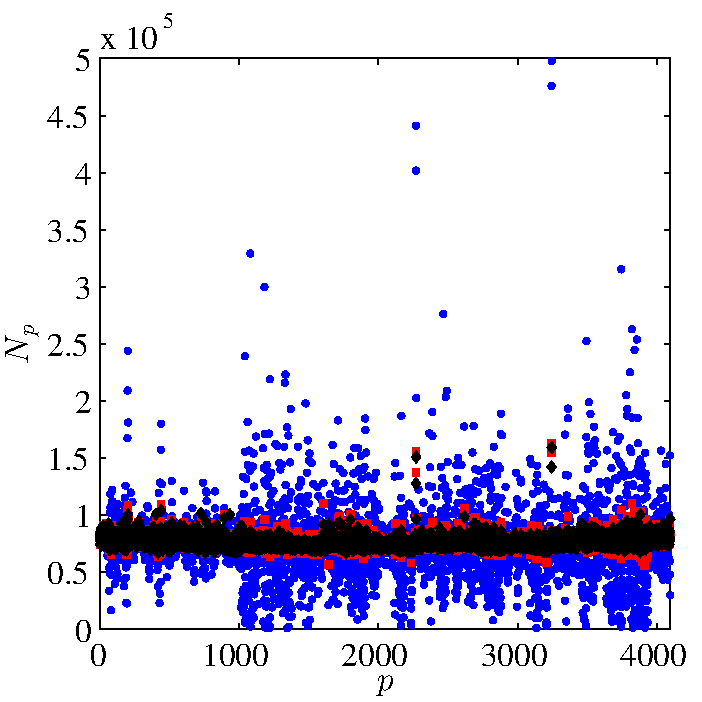
\includegraphics[width = 0.3 \textwidth] {figures/host_large_point_first_4096.pdf}  \label{fig:communication_4096_pf}}
		\subfigure[]{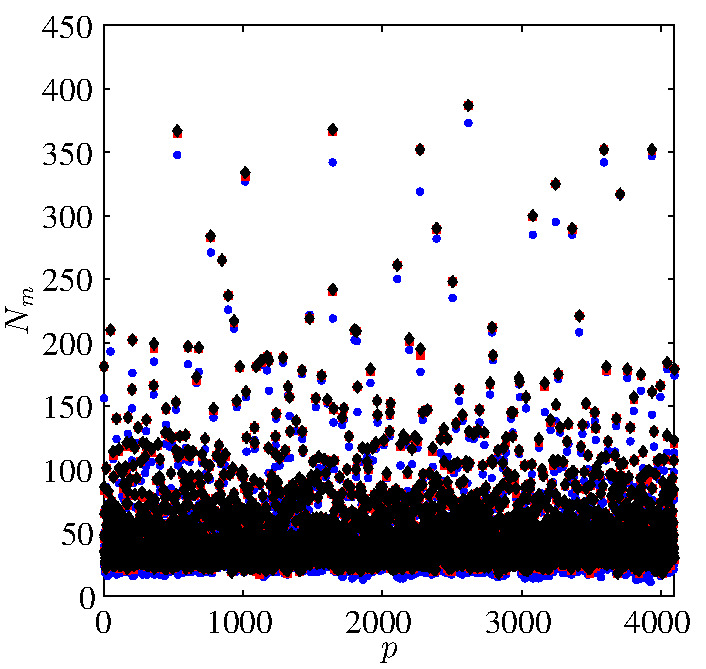
\includegraphics[width = 0.3 \textwidth] {figures/host_large_message_first_4096.pdf}\label{fig:communication_4096_mf}}
		\subfigure[]{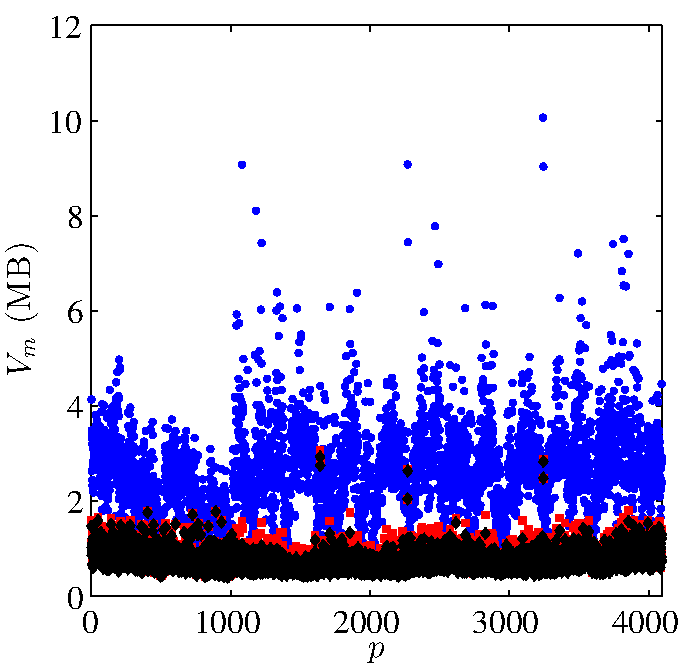
\includegraphics[width = 0.3 \textwidth] {figures/host_large_volume_first_4096.pdf} \label{fig:communication_4096_vf}}
		\\
		\subfigure[]{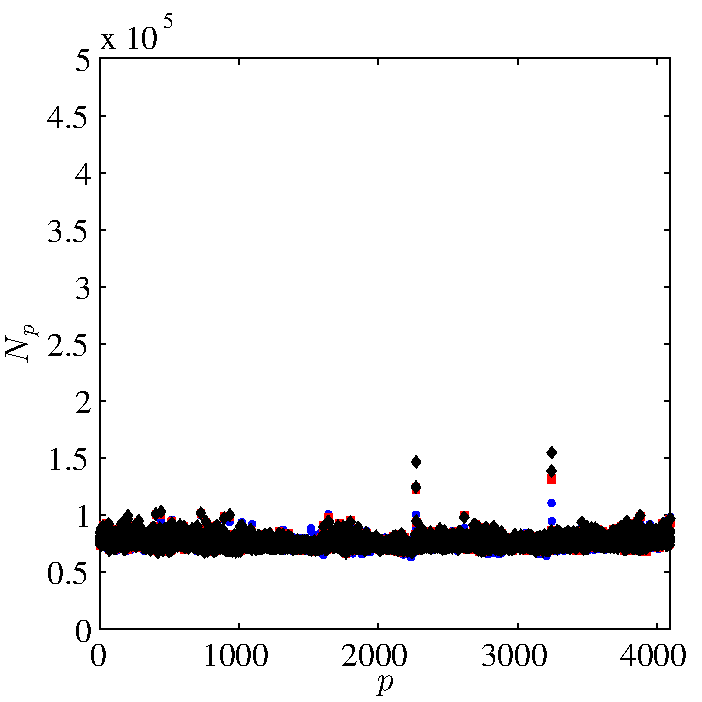
\includegraphics[width = 0.3 \textwidth] {figures/host_large_point_last_4096.pdf}   \label{fig:communication_4096_pl}}
		\subfigure[]{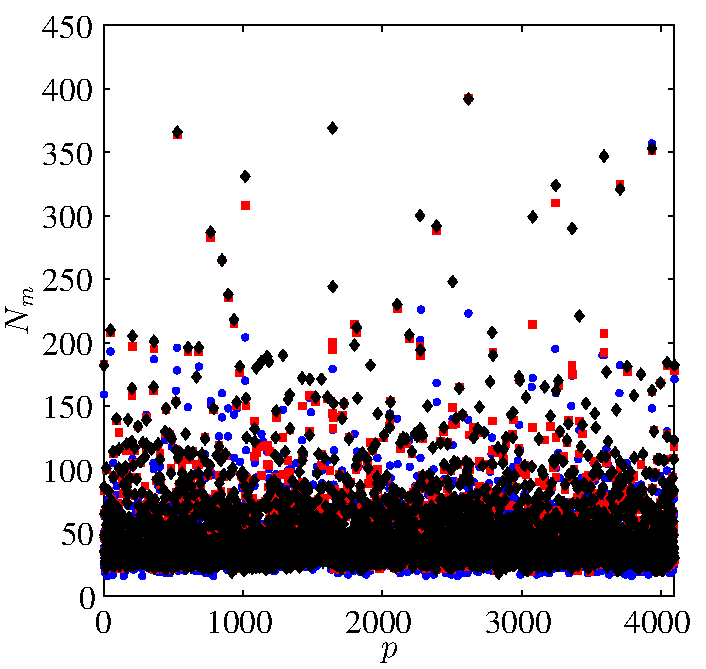
\includegraphics[width = 0.3 \textwidth] {figures/host_large_message_last_4096.pdf} \label{fig:communication_4096_ml}}
		\subfigure[]{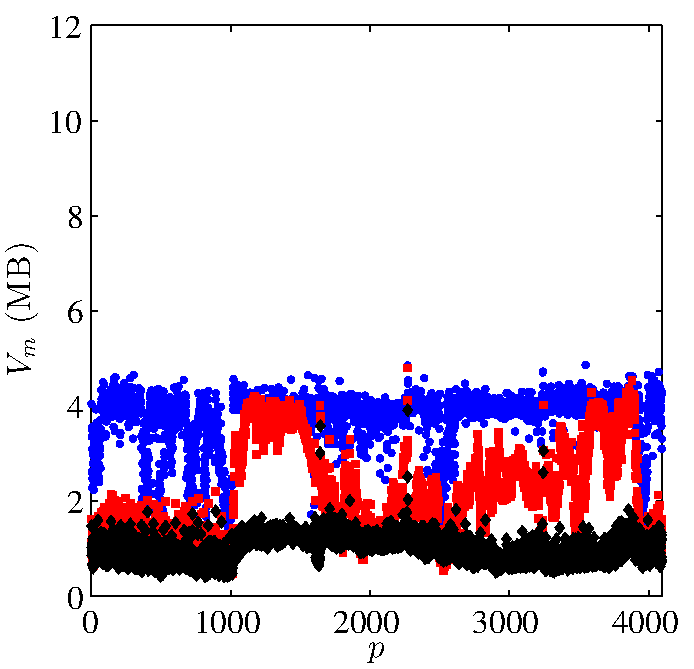
\includegraphics[width = 0.3 \textwidth] {figures/host_large_volume_last_4096.pdf}  \label{fig:communication_4096_vl}}		
	\end{center}
	\caption{Performance indicators of the first (top row) and last (bottom row) sub-iterations of the semi-Lagrangian algorithm for the level-set advection on 4096 processes with $\text{CFL} = 1$ (\drawdiamond{black}), $\text{CFL} = 10$ (\drawsquare{red}), and $\text{CFL} = 100$ (\drawcircle{blue}). Increasing the CFL number causes load imbalance during interpolation (a) and increases the communication volume (c). However, the CFL number does not seem to appreciably affect the number of messages sent by the processes (b). During the last semi-Lagrangian sub-iteration, the initial grid $G_0$ (cf.\ Algorithm \ref{alg:semi-lagrangian}) is very close to the final grid. As a result, the load imbalance is considerably improved (d). Curiously, however, the communication pattern does not seem to be change much between first and last sub-iterations (e,f).}
	\label{fig:communication_4096}
\end{figure}

\begin{table}[htbp]
	\centering
	\resizebox{\columnwidth}{!}{
	\begin{tabular}{|c|c|cccc|cccc|}
	\hline
	\multirow{2}{*}{CFL} & \multirow{2}{*}{Metric} & \multicolumn{4}{|c|}{First sub-iteration} & \multicolumn{4}{|c|}{Last sub-iteration} \\
	\cline{3-10}
											 & 												 & min & max & avg & stddev 					   & min & max & avg & stddev 						\\
	\hline
	\multirow{3}{*}{1}   & $N_p$        & 6.67E+04 & 1.59E+05 & 7.57E+04 & 4.86E+03 & 6.69E+04 & 1.55E+05 & 7.57E+04 & 4.73E+03 \\
										   & $N_m$ 			  & 18 			 & 387 		  & 47.55 	 & 31.72 		& 18 			 & 392 			& 47.55 	 & 31.19 		\\
										   & $V_m$ (MB)   & 4.01E-01 & 2.93E+00 & 7.25E-01 & 1.95E-01 & 4.13E-01 & 3.91E+00 & 9.68E-01 & 2.62E-01 \\
										   & $T_{\max}$ (s) & \multicolumn{4}{|c|}{6.96E-01}						& \multicolumn{4}{|c|}{3.67E-01}						\\
	\hline
	\multirow{3}{*}{10}  & $N_p$        & 5.56E+04 & 1.63E+05 & 7.57E+04 & 6.07E+03 & 6.65E+04 & 1.33E+05 & 7.57E+04 & 4.50E+03 \\
										   & $N_m$ 			  & 17 			 & 387 		  & 46.73 	 & 31.78 		& 19 			 & 393 			& 46.68 	 & 27.93 		\\
										   & $V_m$ (MB)   & 4.01E-01 & 3.06E+00 & 8.40E-01 & 2.21E-01 & 4.40E-01 & 4.80E+00 & 2.14E+00 & 9.88E-01 \\
											 & $T_{\max}$ (s) & \multicolumn{4}{|c|}{7.55E-01}						& \multicolumn{4}{|c|}{3.30E-01}						\\
	\hline
	\multirow{3}{*}{100} & $N_p$        & 8.28E+02 & 4.98E+05 & 7.57E+04 & 3.14E+04 & 6.30E+04 & 1.10E+05 & 7.57E+04 & 4.20E+03 \\
										   & $N_m$ 			  & 11 			 & 373 		  & 41.18 	 & 30.85 		& 16 			 & 357 			& 41.77 	 & 22.66 		\\
										   & $V_m$ (MB)   & 5.28E-01 & 1.01E+01 & 2.65E+00 & 9.24E-01 & 9.76E-01 & 4.86E+00 & 3.78E+00 & 5.69E-01 \\
											 & $T_{\max}$ (s) & \multicolumn{4}{|c|}{9.25E-01}						& \multicolumn{4}{|c|}{3.55E-01}						\\
	\hline
	\end{tabular}
	}
	\caption{Detailed load balancing and communication information for the advection test for $\text{CFL} = 1$, $\text{CFL} = 10$, and $\text{CFL} = 100$. Here $N_p$ is the number of interpolation points, $N_m = S + R$ is the number of sent ($S$) and received ($R$) messages, and $V_m$ is the total communication volume in megabytes (MB). Note how increasing the CFL number causes load imbalance and increases the communication volume while it does not affect the number of messages sent and received during a sub-iteration of the semi-Lagrangian step.}
	\label{tab:communication}
\end{table}

\subsection{Reinitialization} \label{section::scaling_reinitialization}

Finally we present the scaling results of our parallel reinitialization algorithm where we extensively make use of Algorithm \ref{alg:overlap} for overlapping the computations with the communications when computing spatial derivatives. Our test consists in computing the signed distance function to a collection of 100 spheres, whose radii and centers are chosen randomly. The test is performed on a small, level-8 Octree with about 21M and a larger, level-10 Octree with about 337M grid points. In both cases the forest is built on a $3\times3\times3$ macro-mesh. Figure \ref{fig:reinit} illustrates that our reinitialization algorithm, and in particular the overlapping strategy presented in Algorithm \ref{alg:overlap}, scales very well (cf.\ Table \ref{tab:scaling_reinit}). In general we expect similar scaling results for any local, finite-difference based calculations on Octrees that can efficiently utilize Algorithm \ref{alg:overlap}. 
\begin{figure}
\centering
\subfigure[]{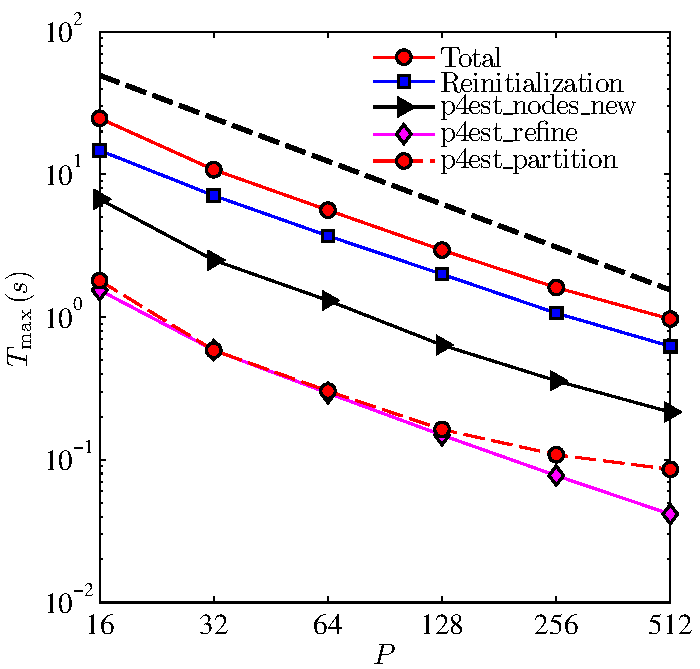
\includegraphics[width=0.48\textwidth]{figures/Reinit_Small.pdf}}
\subfigure[]{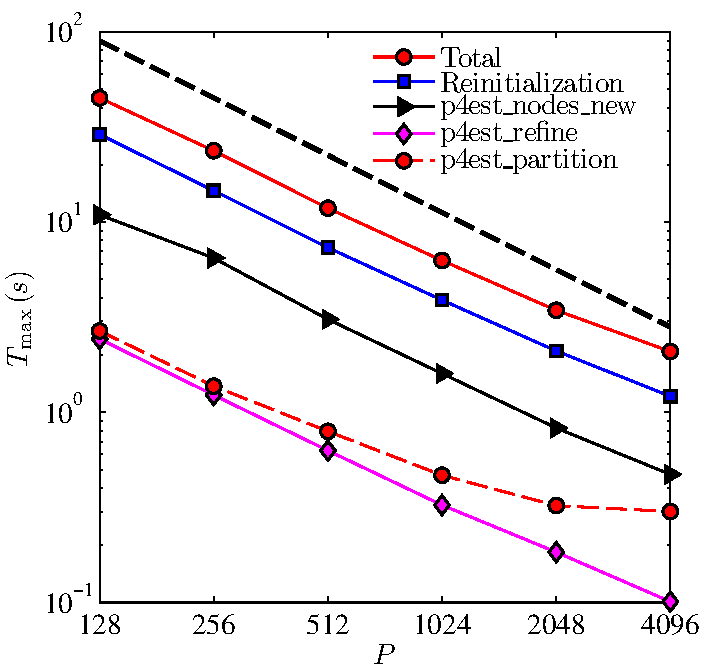
\includegraphics[width=0.48\textwidth]{figures/Reinit_Large.pdf}}
\caption{Scalability of the reinitialization test for a small (left) and large (right) Octree with roughly 21M and 337M grid points, respectively. The black dashed line represents ideal scaling. Excellent results are obtained in both cases, illustrating the scalability of the overlapping strategy (cf.\ Algorithm \ref{alg:overlap}).}
\label{fig:reinit}
\end{figure}

\begin{table}
\centering
	\begin{tabular}{|l|c|cccccc|}
	\hline
	\multirow{2}{*}{Small Test} & $P$ & 16      & 32      & 64      & 128     & 256    & 512 \\ 	                            
	                            & $e$ & $100\%$ & $115\%$ & $110\%$ & $105\%$ & $96\%$ & $80\%$ \\
	\hline
	\multirow{2}{*}{Large Test} & $P$ & 128     & 256     & 512     & 1024    & 2048   & 4096 \\ 	                            
	                            & $e$ & $100\%$ & $95\%$ & $95\%$ & $89\%$ & $82\%$ & $67\%$ \\
	\hline
	\end{tabular}
	\caption{Parallel efficiency of the total runtime for the reinitialization test based on the lowest number of processes for each test.}
	\label{tab:scaling_reinit}
\end{table}
